\section{\projectName}\label{sec:projectDesign}
\subsection{Overview}
As described in section~\ref{sec:introduction}, the goal of this project is to reduce the amount of information presented to the developer, to reduce the overload that is introduced by the amount of information that is readily available.

In order to do so, we have developed \projectName, which allows the user to choose the amount of information required in a page. 

\subsection{Architecture}
The project has two main components:
\begin{itemize}
\item \textbf{Chrome Web Extension}\\
Used to gather the information contained in a page by following the rules set up for a certain domain, as well as controlling the amount of information currently displayed
\item \textbf{Web Service}\\
Instead of relying on the end user's device to perform the calculations to determine the degree of centrality of each component, a web service was developed.
\end{itemize}

These two components interact with each other, in a typical client-server architecture, as shown in figure \ref{fig:architecture}.
\begin{figure}[H]
\centering
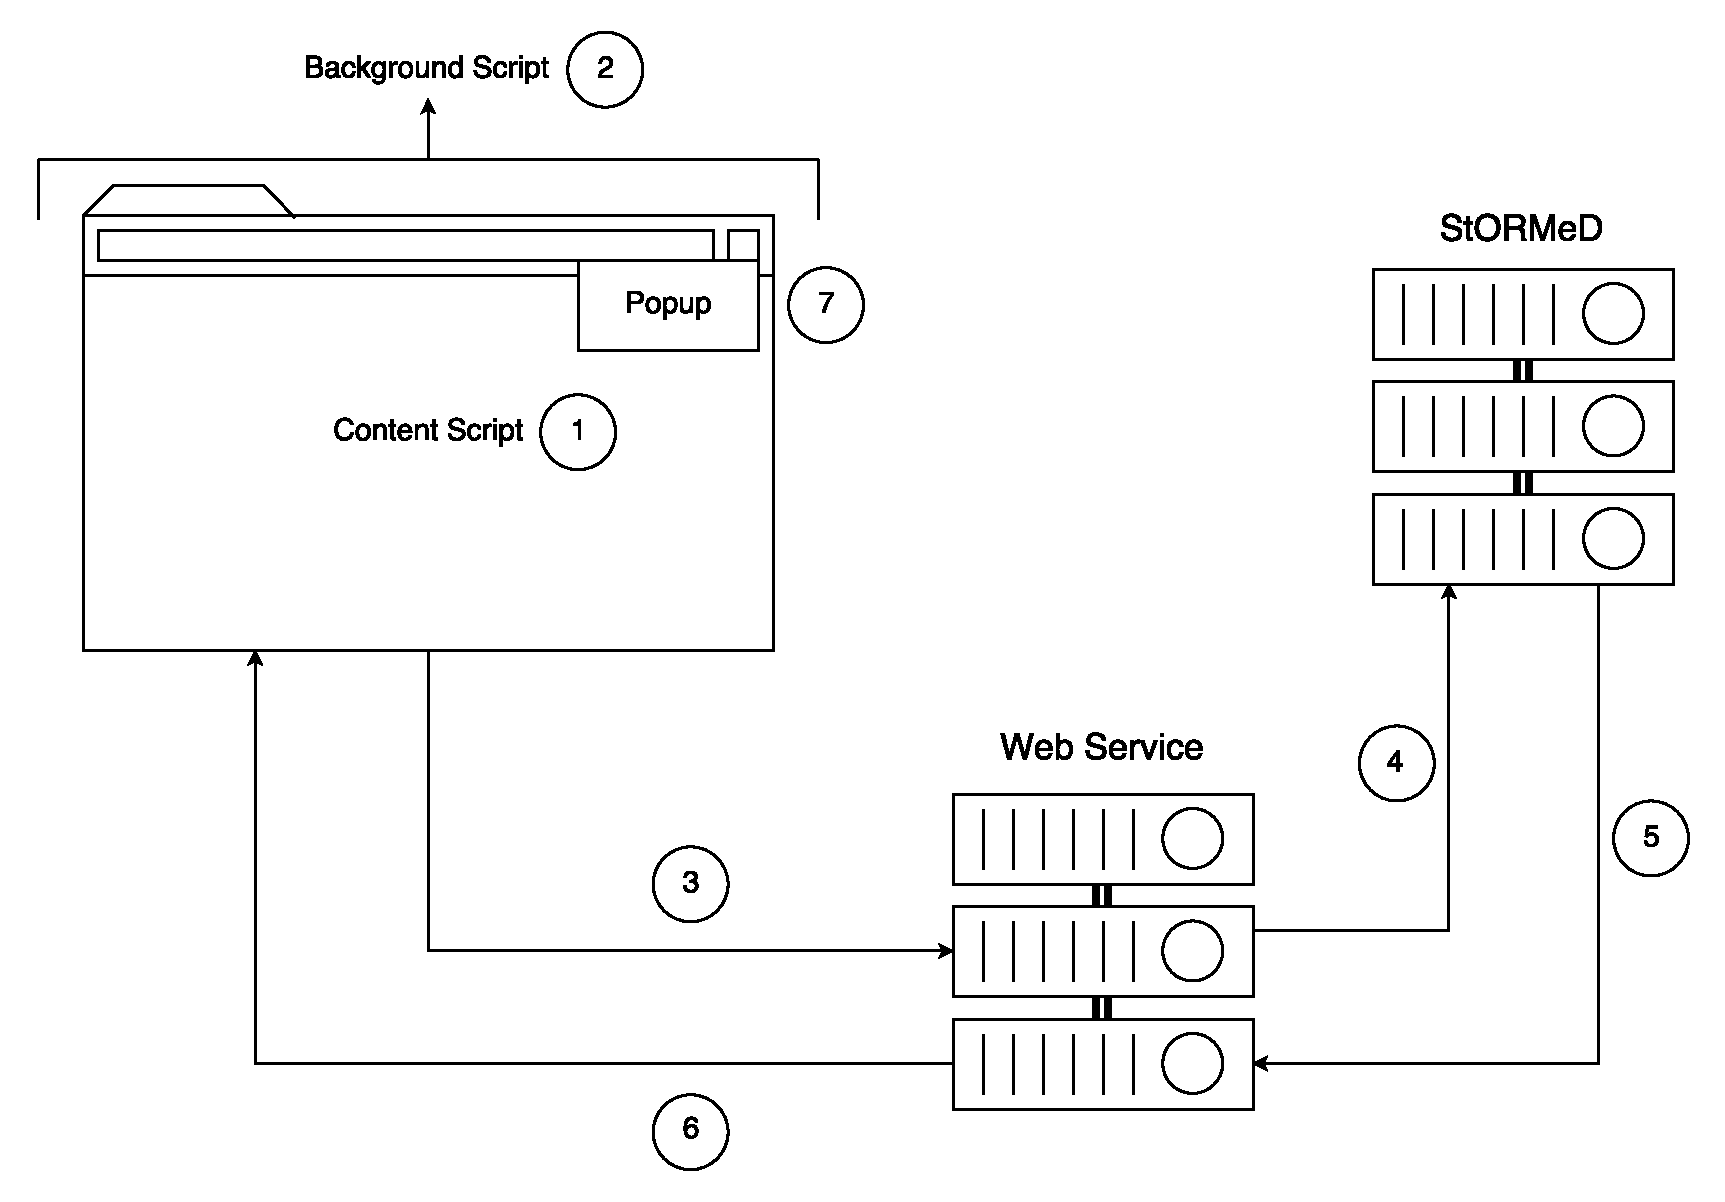
\includegraphics[scale=0.4]{Figures/Architecture}
\caption{Architecture of \projectName}
\label{fig:architecture}
\end{figure}
Each of these numbers will be explained in a later section. In the next few sections, we will analyse each component, and its specific tasks.

\subsubsection{Parser}
The first step consists in collecting the information currently being displayed, which happens when the page has finished loading its content. As previously discussed\todo{Add reference}, one of the main challenges of this project was to handle the wide variety of structures among webpages, being as each page tends to use the same constructs but widely differ in the implementation. This hurdle was solved by implementing a parser for each of the domains for which the information was needed. 

\begin{figure}[H]
\centering
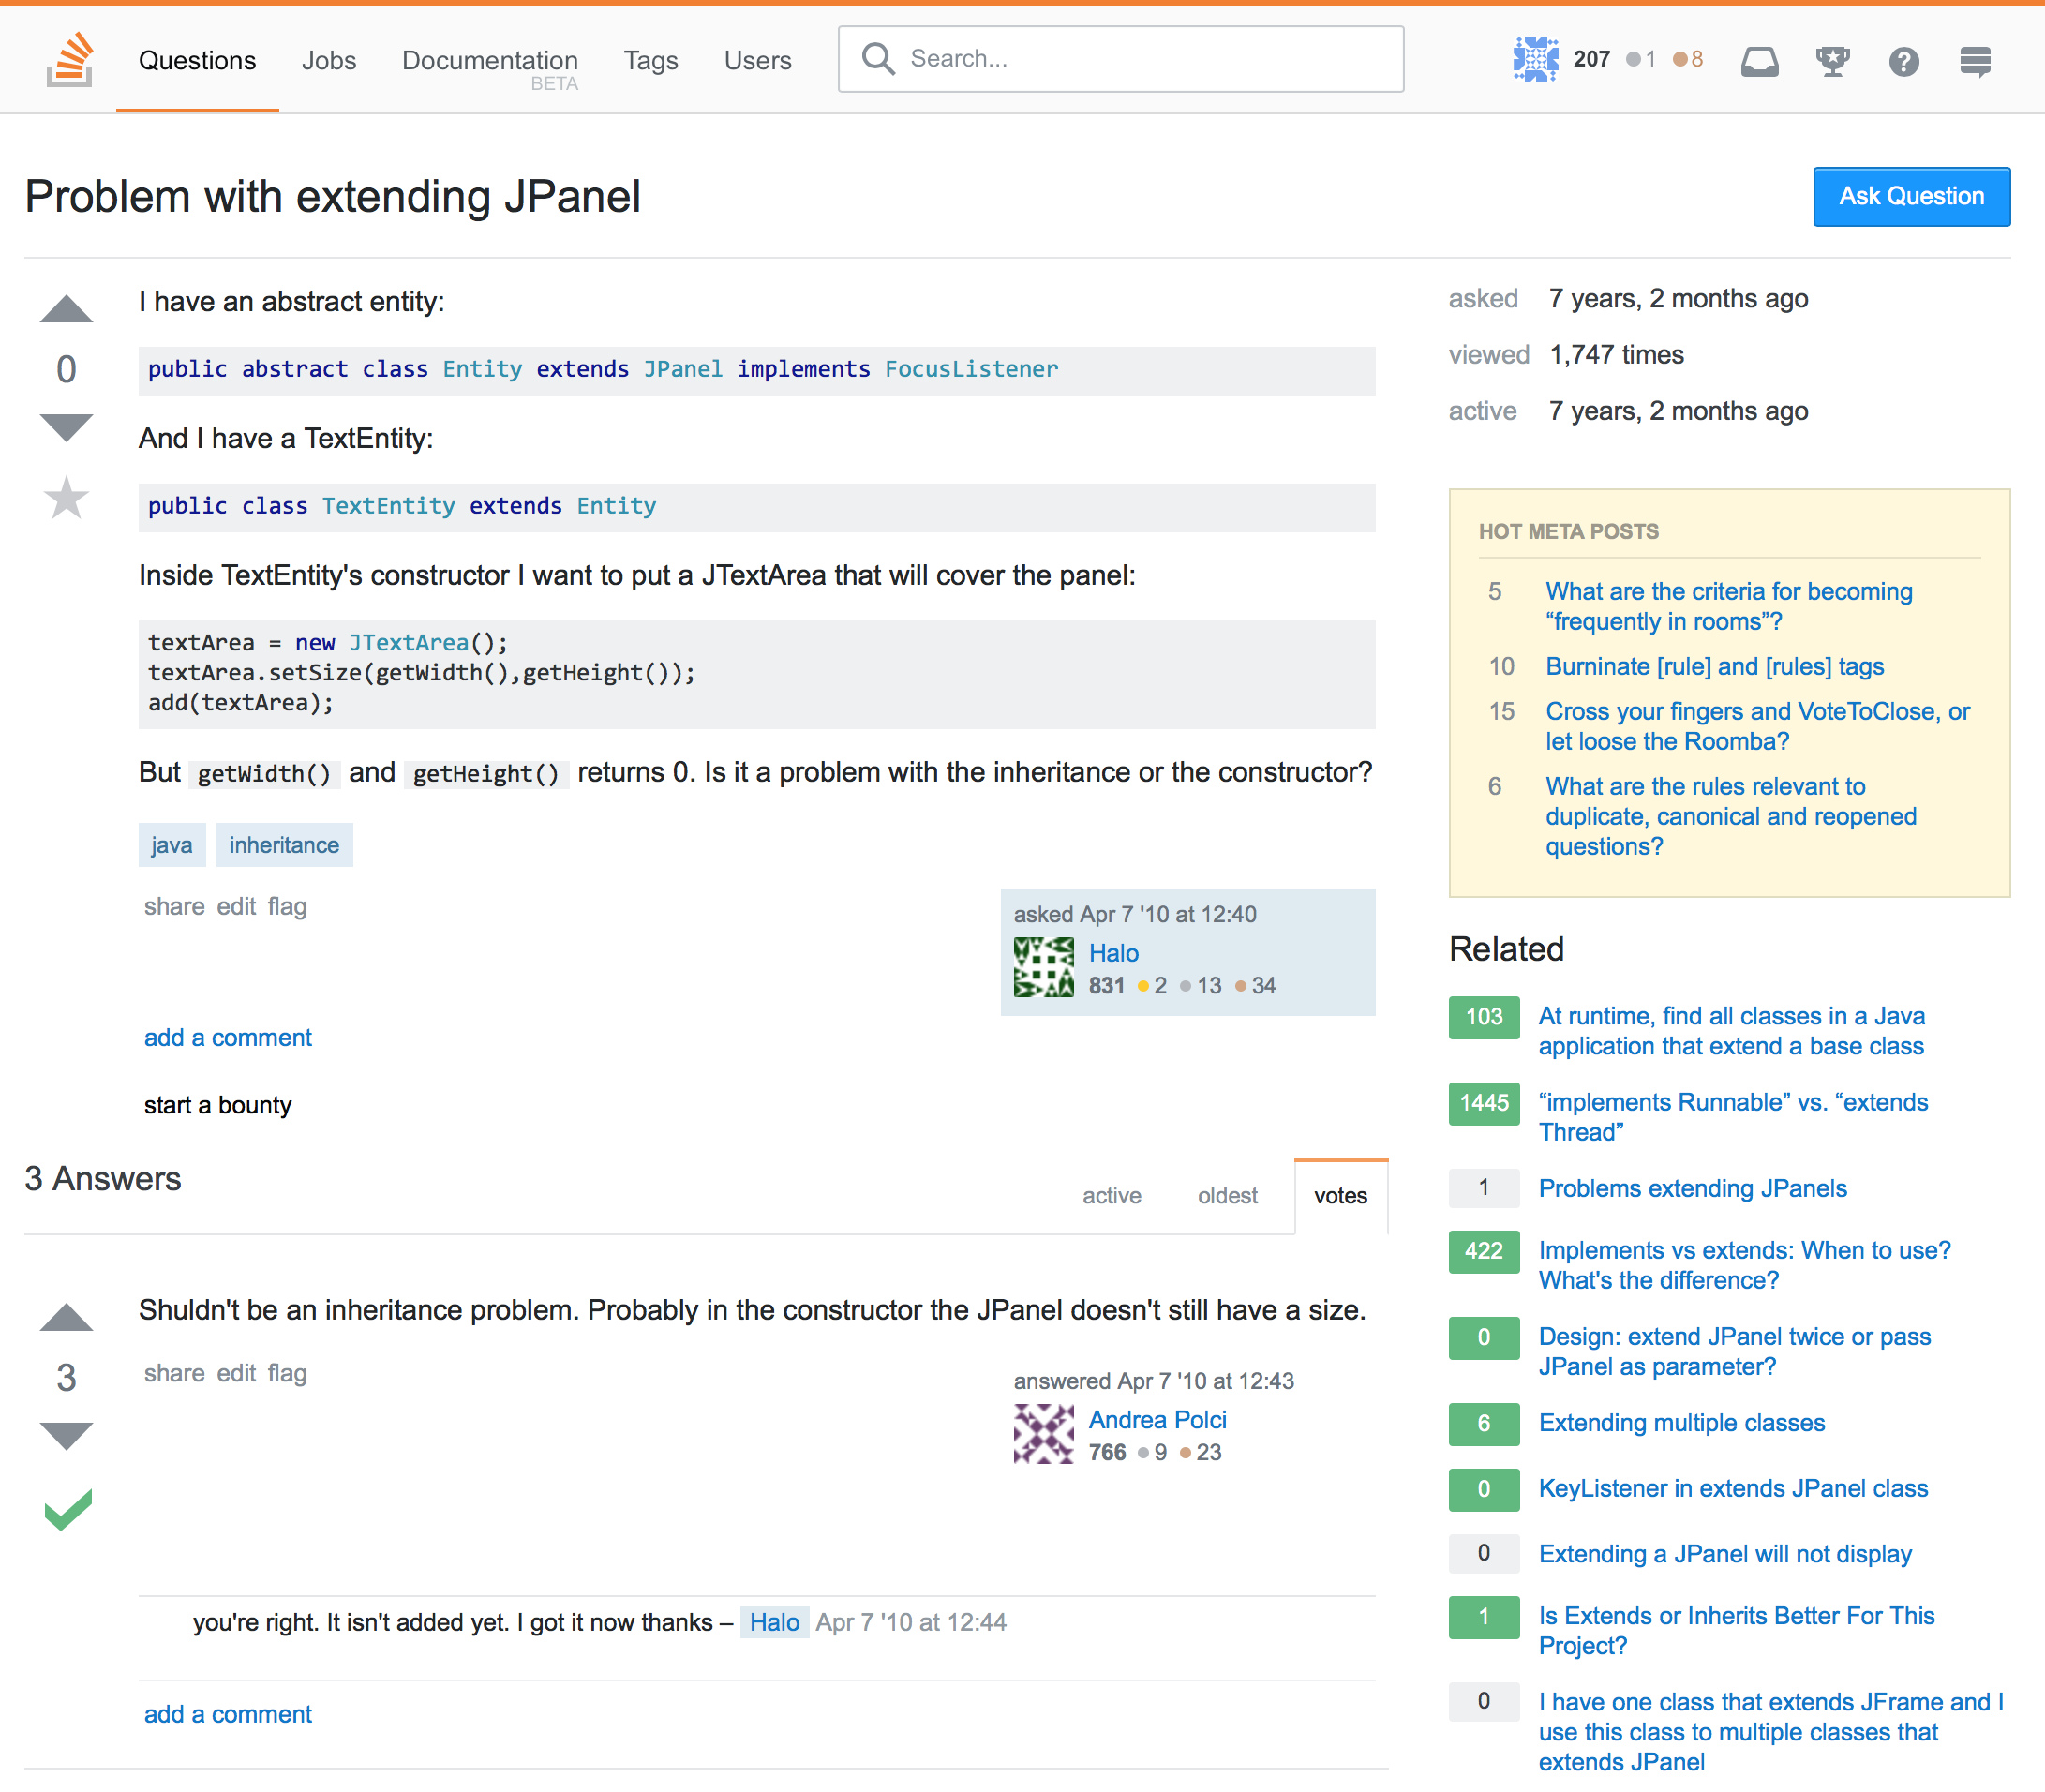
\includegraphics[scale=0.3]{Figures/SOConv}
\caption{A typical StackOverflow conversation}
\label{fig:soConv}
\end{figure}

Figure \ref{fig:soConv} represents the structure of a StackOverflow conversation. It is easy to see that there is a set structure which consists of a question, and $0$ or $n$ answers. Therefore our parser needs to first obtain the question, more specifically the paragraphs that make up such question, and then repeat the task for each of the possible answers. 

In order to classify these pieces of information, we introduce the notion of an information unit. An information unit is a piece of content extracted from a page, which contains either text or code. The distinction has to be made when the content is extracted, in order to keep the integrity of code in such a way that it may be used later on by a simple copy and paste approach. 

To ease the process of writing a parser, an abstract parser was created, with a few models to accompany the methods. Being as the parser has to live inside of the browser extension, the language sed to write such a program is JavaScript. Although a pretty complete programming language \todo{CRINGE}, the current version as of writting this document is ES5\todo{Sure?}, which does not yet support features such as classes, inheritance, and more. Being as our implementation is supposed to be abstract, meaning that for each domain this parser can be extended, we needed a language that could support inheritance. After a bit of research, the choice ended up being TypeScript\footnote{\url{https://www.typescriptlang.org}}, a language developed by Microsoft which is a typed superset of JavaScript that compiles to plain JavaScript. This ensured that compatibility would not be an issue, while providing multiple useful features. 

\begin{figure}[H]
\centering
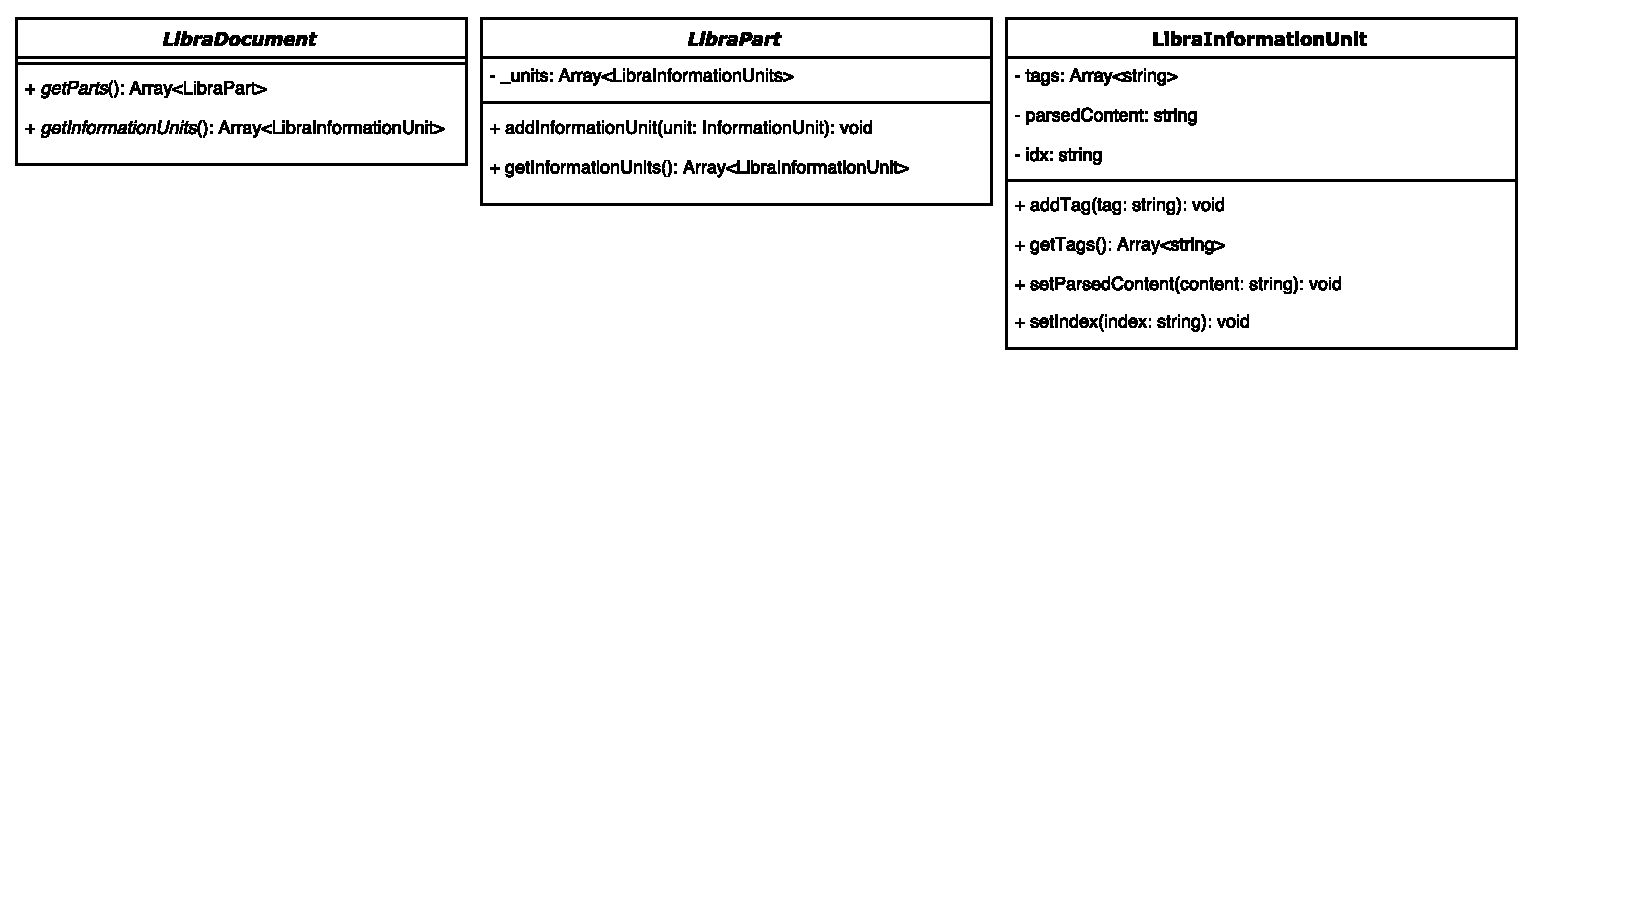
\includegraphics[scale=0.5]{Figures/ClassUML}
\caption{Abstract parser class diagram}
\label{fig:abstractParserClassDiagram}
\end{figure}


We started by defining the models that would be needed to parse a page. A document diagram can be found in Figure \ref{fig:abstractParserClassDiagram}.

The ``root'' model is called \ts{LibraDocument} which provides the main methods that will be called by the extension, namely \ts{parse()} and \ts{getInformationUnits()}. Then, the information unit is defined, which encapsulates the data required to run the analysis. The last piece is \ts{LibraPart}, which allows us to separate the multiple parts of a document. As an example, consider the previously shown StackOverflow conversation. We could divide the question and the answers in two separate parts, which themselves contain other parts (i.e. the possible answers). 

\begin{figure}[H]
\centering
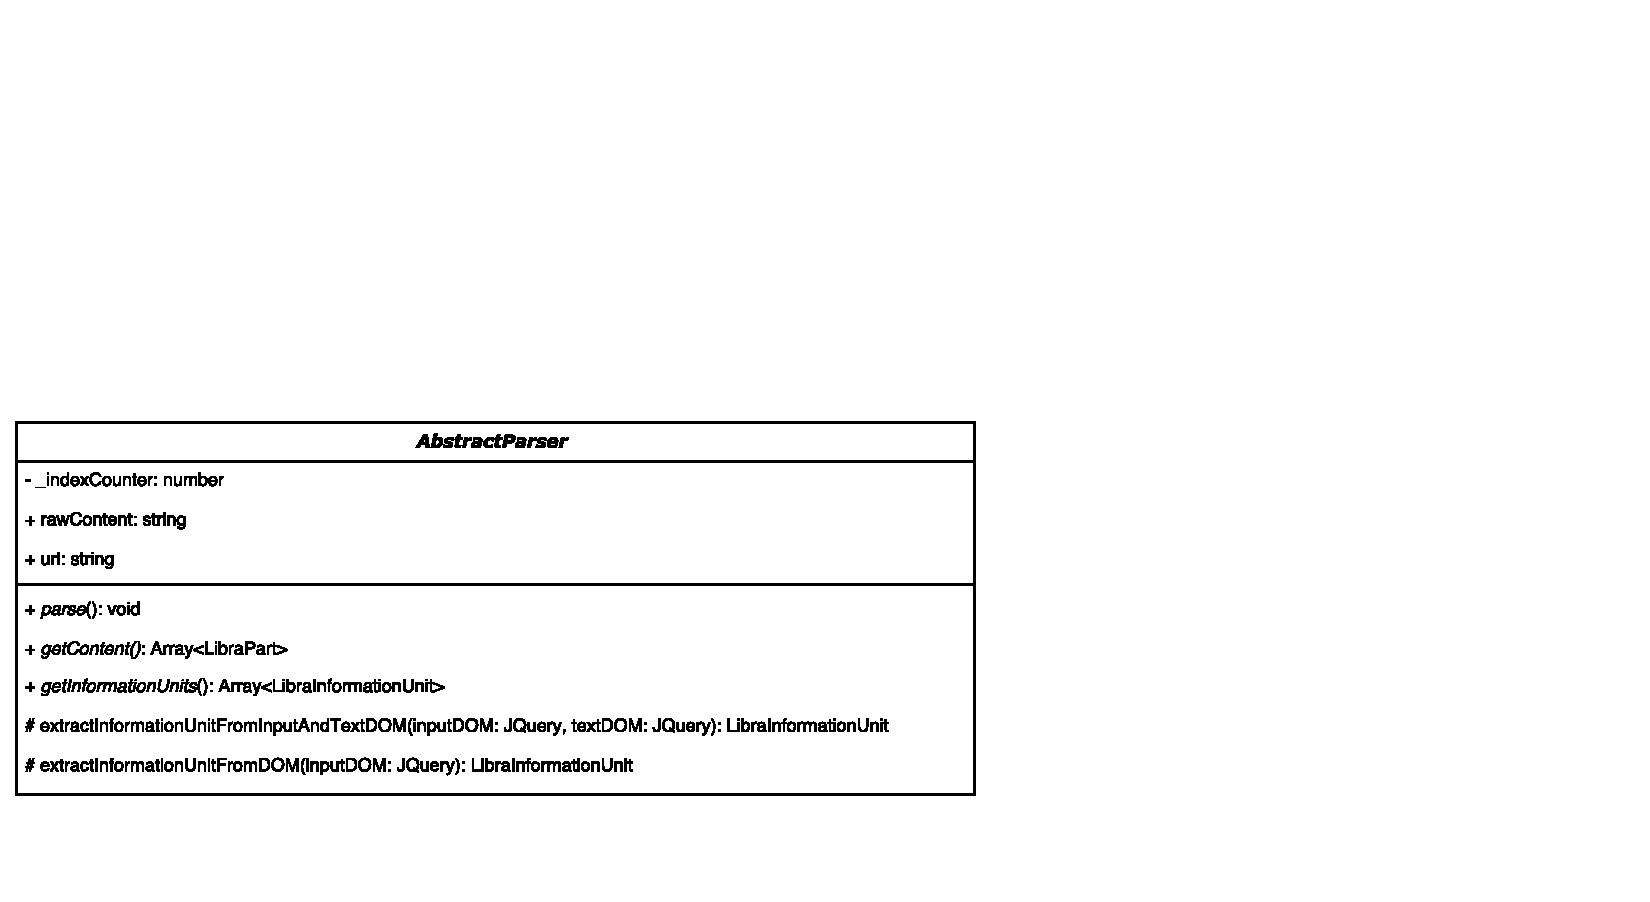
\includegraphics[scale=0.5]{Figures/AbstractParserUML}
\caption{Abstract parser}
\label{fig:abstractParserDiagram}
\end{figure}

These models are then used in the abstract parser, for which the diagram is show in figure \ref{fig:abstractParserDiagram}. This way the developer writing a new parser has to simply extend the different methods and models, quickly creating a new parser which the extension is able to understand and use. 

A remark ha to be made about the \ts{extractInformationUnitFromDOM} and \ts{extractInformationUnitFromInputAndTextDOM} methods. These two methods were created to keep the way that the data is extracted consistent among multiple parser implementations. The two methods are almost identical, and work in the following way:

\begin{enumerate}
	\item A small marker, comprised of the URL hash combined with the current counter inside the document is injected into the HTML tags containing the information, like so:
\begin{htmlcode}
<pre class="lang-java prettyprint prettyprinted" libra_idx="-656298628_0000000001">
    ...
</pre>
\end{htmlcode}
\item The counter is then increased
\item The type of the content, text or code, is identified and attached inside of the information unit
\item The information unit is returned to the developer
\end{enumerate}
The reason why we are injecting the index is quite simple. In order to identify the unit to which a certain degree belongs to, we need to leave small traces such as this index, being as the service does not return the parsed text, but only the index and degree. This procedure is explained more in details in section \todo{Needs ref}. The index construction needed to abide to certain constraints, namely the ability of being unique inside a document, as well as when doing multiple document summarisation. In the end, the approach we chose was as follows:
\[
\text{\texttt{Hash of url + "\_" + 10 digit padded index}}
\]
Although hashing may introduce cases where the produced hash is not unique, the probability of such an event occurring was small enough to be ignored.


By creating the two methods in \ts{LibraDocument} as abstract, each parser can implement their own, while allowing the extension to call the same methods, regardless of the page being viewed (and hence parser being used), while effectively providing a common interface to the parser. 

The execution of the parser is performed once the loading of the page is completed, which itself fires the request to the web service, discussed in this next section.

\subsubsection{Web Service}
The second main component of this project consists in a web service, that takes the information units given by the extension, and returns the degree of centrality for each of the information units. This service was written in Scala, using the Play framework. Most of the code is written in a functional way\todo[inline]{Can this be said?}, which proved to be quite the challenge but very satisfying when things were working correctly. 

The service has the following routes:

\begin{itemize}
\item \texttt{GET /register}\\
Used to register the user to the service. This is needed as to identify the user in all subsequent calls to the service. The response is a 32-character string, which contains both numbers and letters. Once the user registers, a graph is created unique to this id, allowing for subsequent information units to be added, and therefore the ranking to be performed depending on the entire graph, not only the current units being analysed.
\item \texttt{POST /rank}\\
This path is used to rank the current units extracted from a document. By supplying the url of the webpage, the units, and the user id header, the service will return the units with a degree of centrality. 
\texttt{GET /all}\\
Returns the entire graph for a certain user, with all units associated with their degree of centrality.
\end{itemize}

\noindent In figure \ref{fig:architecture} the entire architecture is shown. An example workflow\todo{This does not sound good} is as follows:
\begin{enumerate}
\item User install the extension, opens it for the first time which prompts the registration procedure
\item The user id is stored in storage, for later use
\item The user navigates to a known page, which fires the content script's parsing process (Label 1)
\item Once parsing is completed, the background script takes over and prepares the data to be sent (Label 2)
\item The data is sent to the web service, which starts processing (Label 3) \label{item:serviceRequest}
\item The service sends a part of the data over to the island parser (Label 4)
\item Once the data is returned (Label 5), if it is the first request for that particular user, the graph is created
\item The nodes are added to the graph, and ranking starts \label{item:serviceRank} 
\item Once completed, the data is returned to the background script, which notifies the popup that the data is ready (label 6) \label{item:serviceReturn}
\item The popup prepares itself, and the user ca now interact with it (Label 7)
\end{enumerate}

In this section we are going to focus on points \ref{item:serviceRequest}, \ref{item:serviceRank}, and \ref{item:serviceReturn}. When the extension makes the request, a few pieces of informations are needed. The following is an example of the request:
\begin{jsoncode}
POST /rank
Content-Type: application/json
X-Libra-UserId: SsrktS2vrGPpHaAkYMsVDPo4qN6i38ei

{
  "units": [
    {
      "idx": "-656298628_0000000001",
      "parsedContent": "Creating an instance of a class:",
      "tags": [
        "plaintext"
      ]
    },
    {
      "idx": "-656298628_0000000002",
      "parsedContent": "MyObject myObject = new MyObject();",
      "tags": [
        "code"
      ]
    }
  ],
  "url": "http://www.MyAwesomeWebsite.rocks"
}
\end{jsoncode}

As we can see, the request requires the content type, the user id when registration happens, as well as the units with the url. 


Once the units are received, the service will fire a request for each of the units to the StORMeD\cite{Ponz2015b} service. This service is an island parser, which will allow us to construct the full AST from a certain unit. 

The service will then add the nodes to the graph, and start calculating the degree by using a library called Signal/Collect\cite{Stutz:2010:SGA:1940281.1940330}, which allows the processing of large graphs in a really quick way. By describing the HoliRank algorithm using the provided syntax, the library handles the calculations returning the degree of centrality for a certain unit. The results are then returned to the user in the following format:
\begin{jsoncode}
{
  "units": [
    {
      "idx": "-656298628_0000000001",
      "degree": 0.5,
      "url": "http://www.MyAwesomeWebsite.rocks"
    },
    {
      "idx": "-656298628_0000000002",
      "degree": 0.5,
      "url": "http://www.MyAwesomeWebsite.rocks"
    }
  ]
}
\end{jsoncode}

This information is then used by the extension to associate the index with its degree, which is then used to decide which units have to be hidden and which have to be shown depending on the value chosen by the user. This is explained in details in the next section.

\subsection{Chrome Extension}
As previously stated, in order to parse the content of a certain page, send it to the service, and then manipulate it, a Chrome extension was created. The extension encapsulates three main components:
\begin{itemize}
\item \textbf{Content Script}\\
The content script has the task of loading the available parser, as well as using such parser. Once this is completed, the data is handed over to the background script.
\item \textbf{Popup}\\
The popup is the only piece of this project which a user can see. It is the main point of interaction between the user and the project. She has the ability to choose the amount of information that has to be displayed. 
\item \textbf{Background script}\\
The background script has the task of connecting the content script with the popup. 
\end{itemize}
Before we go any further, one must understand how a Chrome extension works. As with our implementation, an extension usually consists of three main components as described above. These components have different restrictions regarding what data they can access, how they are instantiated, and when they are destroyed. 

The background script is persistent, meaning it stays alive for the duration of the session, and has the ability to make HTTP requests but has no access to the content on the page, or the content of the popup. On the other hand, the content script has the ability to access the content, but no access to the popup. Last but not least, the popup is recreated every time the user clicks on the icon, and has no access to the content. This means that the three components have to communicate to each other, by means of message passing. 

Each of these components has the ability to send and receive messages, and react accordingly. This was useful when, for example, the user had just registered to the service. Each component has its own localStorage, but the user id had to be used by multiple components which created an issue regarding where to store it. In the end message passing was used and a common local storage was chosen, this being the background script's storage as this component was always listening and active.


As we have seen in the previous section, the service returns the payload containing the different degrees of each unit. It is the task of the extension as a whole to process this information, and make it usable to the user. This is achieved by sorting the payload data, and adding in each of the units currently on the page a sort order index, as follows:
\begin{htmlcode}
<pre class="lang-java prettyprint prettyprinted" libra_idx="-656298628_0000000001" sortorder="15">
	...
</pre>	
\end{htmlcode}
Once this manipulation is complete, the popup updates its view, and shows a range slider, allowing the end user to choose the percentage of the information that she may want to be displayed. Every time the value of the slider changes, the popup fires a message, calling into action the content script which will hide or show the units depending on their sort order. The interface is shown in figure \ref{fig:chromeExtensionInterfaceScreenshot}

\begin{figure}[H]
\centering
\missingfigure{Screenshot of the extension with the popup open and bar dragged}	
\caption{Interface of the Chrome extension}
\label{fig:chromeExtensionInterfaceScreenshot}
\end{figure}

Another feature of the extension, is the ability of generating a page containing all the units that have been visited by a certain user. If the user clicks on the summary button, a new page is opened containing all of the units, and for each site a range slider is added to choose the amount of information displayed. An additional range slider is added at the top of the page, called a master slider, which controls the amount of information displayed by each site, regardless of the value chosen by each individual slider. This allows the user to consult only the highest ranked units in a website, giving a very quick overview of multiple sites at the same time. The result can be seen in figure \ref{fig:chromeExtensionSummaryScreenshot}

\begin{figure}[H]
\centering
\missingfigure{Screenshot of the Summary	}
\caption{Generated Summary}
\label{fig:chromeExtensionSummaryScreenshot}
\end{figure}
